\begin{figure}[ht!]
    \begin{subfigure}{.5\textwidth}
    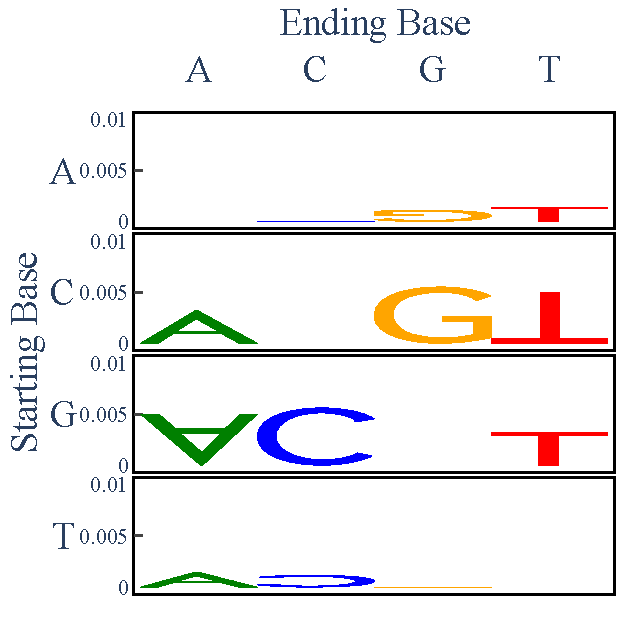
\includegraphics[scale=0.7]{graphics/spectra_Kidney-RCC_Skin-Melanoma.pdf}
    \caption{Kidney-RCC \textit{v.s.} Skin-Melanoma}
    \label{fig:spectra_kidney_skin}
    \end{subfigure}
    ~
    \begin{subfigure}{.5\textwidth}
    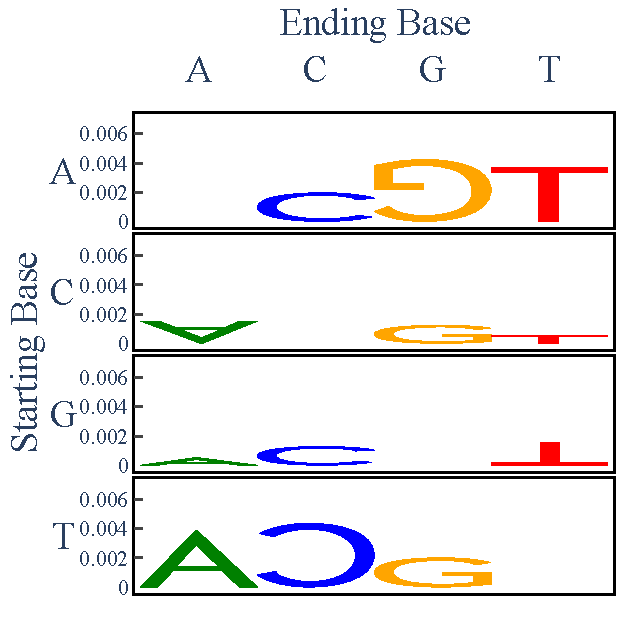
\includegraphics[scale=0.7]{graphics/spectra_Kidney-RCC_Liver-HCC.pdf}
    \caption{Kidney-RCC \textit{v.s.} Liver-HCC}
    \label{fig:spectra_kidney_liver}
    \end{subfigure} \\
    \vspace{0.5cm}
    
    \begin{subfigure}{.5\textwidth}
    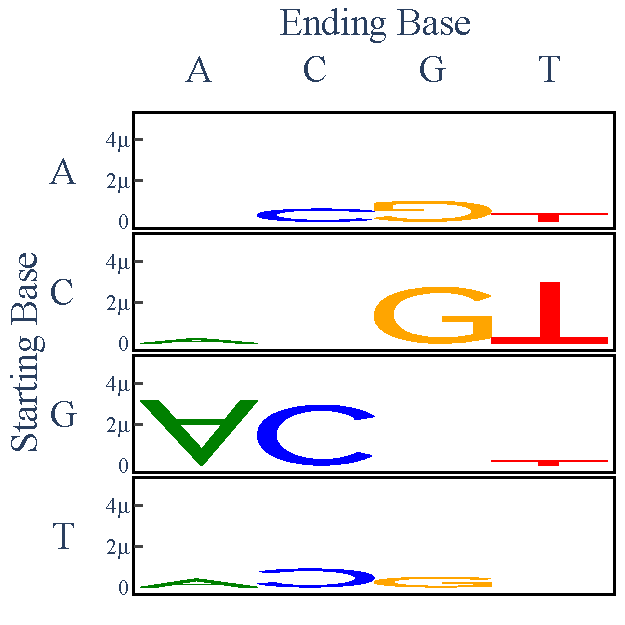
\includegraphics[scale=0.7]{graphics/spectra_CNS-Medullo_CNS-PiloAstro.pdf}
    \caption{CNS-Medullo \textit{v.s.} CNS-PiloAstro}
    \label{fig:spectra_medullo_piloastro}
    \end{subfigure}
    ~
    \begin{subfigure}{.5\textwidth}
    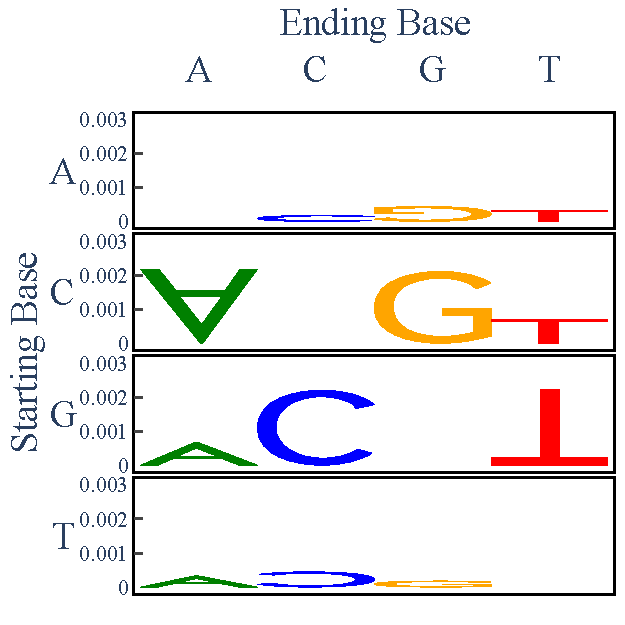
\includegraphics[scale=0.7]{graphics/spectra_CNS-PiloAstro_Lymph-BNHL.pdf}
    \caption{CNS-PiloAstro \textit{v.s.} Lymph-BNHL}
    \label{fig:spectra_piloastro_bnhl}
    \end{subfigure} \\
    \vspace{0.5cm}
\caption{}
    % \caption{\textbf{Base substitutions are promising in discriminating cancers according to $RE$ between cancer pairs.} Similar to Figure \ref{fig:spectra}, for each panel, each row contains the measure of information $RE$ derived from a pair of GLMs. The x-axis is the wildtype base; the y-axis is the product of the substitution. The heights of the letters are $RE$'s. An up-orientation indicates an excess while a down-orientation indicates a deficit of the mutation when comparing the (a) Kidney-RCC to Skin-Melanoma, (b) Kidney-RCC to Liver-HCC, (c) CNS-Medullo to CNS-PiloAstro, (d) CNS-PiloAstro to Lymph-BNHL. More comparisons can be found in Figure \ref{fig:apdx_paired_spectra}.}
    \label{fig:paired_spectra}
\end{figure}